\documentclass[12pt,a4paper,conference]{IEEEtran}
%usepackage[backend=bibtex,style=ieee]{biblatex}
\usepackage[authordate,strict,backend=bibtex,babel=other,bibencoding=inputenc]{biblatex-chicago}
\usepackage[thinlines]{easytable}
\usepackage{array}
\usepackage{color}
\usepackage{graphicx}
\usepackage{float}
\bibliography{chicagofile}

\title{{\color{blue}A study on data security and
data usage regarding online
services}}

\author{MD Yamin Haque, Roll No : 1603007\\
MD Al Siam, Roll No : 1603008\\
Department of Computer Science and Engineering\\
Rajshahi University of Engineering and Technology}

\begin{document}
\maketitle

\begin{abstract}

We have to provide our personal data to many online service providers in order to get their services. There arises questions regarding security and safety issues of the data given to the service providing companies. This working paper is a study on how the service providing companies ensure security to the user data. Further, there is study on how companies use data to make their benefit and the impacts of that.
\end{abstract}

\section{Introduction}
In recent years, there have been established a wide range of service providing companies which are internet based. They can get our data when we sign up on their websites. Also, giant companies can follow and track their user’s activities and collects data on user’s behaviors, movements, social relationships, interests, weaknesses and most private moments.\autocite{Wolfie17} 
\\
\\
As online services industry is growing bigger day by day, cyber attacking on data of all kinds of companies has increased. According to the National Cyber Security Alliance 60 percent of small and midsized businesses that are hacked go out of business within six months.\autocite{joe18} Hence, security of data has become a major concern for both the company itself and the users. We will explore on some procedures which are being used to protect data or security on user data.
\\
\\
User data is valuable to companies it tells companies about their audience’s interests. Companies use those data to improve their service as well as to make profit. Common ways to make money with an Internet business include collecting advertising revenue, selling products or services and building an online marketplace. In order to make custom advertising, companies need to use different types of user data like profile data, purchase data, scratch data etc.\autocite{CLINT} This paper will further explore on how companies use and monetize their user data.


\begin{figure}[h!]
  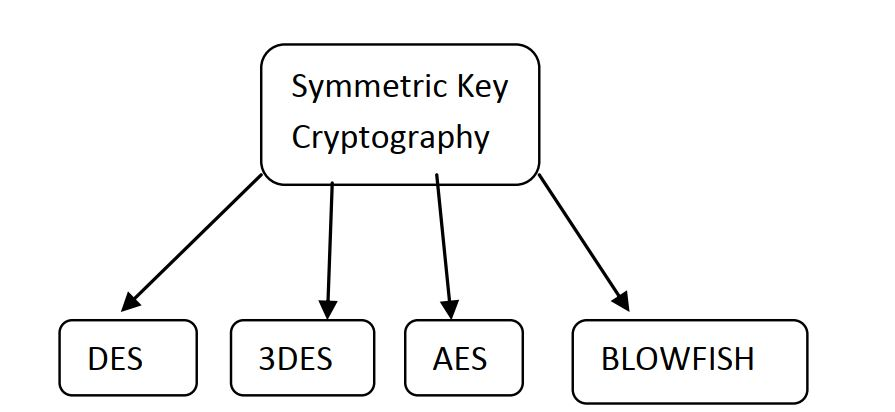
\includegraphics[width=\linewidth]{fig2.jpg}
\end{figure}


\section{General Encryption Algorithms Used to Protect User Data}


The encryption algorithms are used to provide security against unexpected attacks. There are many encryption algorithm used. Some of them are \textbf{DES} (Data Encryption Standard), \textbf{Triple DES} (3DES), \textbf{AES} (Advanced Encryption Standard), \textbf{Blowfish},  \textbf{RSA } etc.\\
\\

\begin{table}[h!]
  \begin{center}
    \caption{Cryptography Algorithms A Comparison}
    \label{tab:table1}
   \renewcommand{\arraystretch}{2.5}
    \begin{tabular}{|c|c|c|c|}
    \hline

      \textbf{Algorithm} & \textbf{Created By} & \textbf{Key Size}& \textbf{Block Size}\\
    
  \hline
   
   DES & IBM in the year 1975 & 56 & 64\\ 
  
\hline

3DES & IBM in the year 1978 & 112 (or) 168 & 64\\

\hline

AES & Joan Daemen and Vincent & 256 & 128\\

\hline

Blow Fish & Bruce Schneier & 32 (or) 448 & 64\\

\hline
    \end{tabular}
  \end{center}
\end{table}



 DES was first introduced by IBM in early 1970s.This was first used by National Institute of Science and Technology, which is under United States Department of Commerce.National Security Agency (NSA) of USA used a modified version of it in 1976.  As the key size of DES is 56-bit key size, which is too small, its security providing quality is low. As 56 bit DES is not capable of protecting the brute force attack, TDES was introduced, which uses three steps DES encryption. Triple DES, also known as 3DES, TDEA (Triple Data Encryption Algorithm)\autocite{barker2017recommendation} was the first algorithm to be disclosed for public usage. It can use 112 bit key size, but due to security issues, NIST uses the 80 bit version, as the 112 bit mode can be attacked by chosen-plaintext or known plaintext attacks.\autocite{merkle1981security} \autocite{van1990known} AES is a block cipher, meaning, the number of bytes that is encrypted is fixed. At present, AES encrypts unit of 16 byte at a time, which is also the minimum number of bytes this method can encrypt at a time. Less than 16 byte texts should be padded. \autocite{berent2013advanced}  AES is also called as Rijndael, which is its original name.\autocite{daemen1999aes} Blowfish encryption algorithm uses 64 bit blocks and 32-448 bit key size. It has not faced any attacks yet.\autocite{laser2016comparative} It was established by Bruce
Schneie in the year 1993 \autocite{malhotra2013study}.

\section{Techniques Used to Prevent Data Leakage by Some Online Services}

\subsection{Facebook}
To prevent the user from various kinds of attacks, this website has developed different types of feature in the backend. One Time Password (OTP) and distant logout feature allows user to get secured when users are not sure about security about their used network or systems. Facebook allows user to strengthen his account’s security by allowing user to change settings at “account settings” section. Now facebook is completely run over https. Facebook messaging service, which is generally done through facebook website, facebook app, facebook messenger, uses end-to-end encryption. This system encrypts message from sender to receiver, and then encrypts again between the server and recipient. Usually only the people with the key to decipher an end-to-end encrypted message are the sender and intended recipient. Facebook also observes unusual activities like a user is logged in from any region and some moments later he is logged in from another region which is so far away from the first region. Facebook also observes violent, unusual or unethical contents uploaded on it and take steps against those posts to keep the environment secured. This website uses conventional captchas which is hard to decode by computer outbreakers. Apart from that, this website uses another ways like sometimes it may ask users to detect another friend’s name or pictures. \autocite{neha16}

\subsection{WhatsApp}
WhatsApp is also a messaging and content sharing service owned by facebook. It has more than one billion monthly users. WhatsApp uses powerful encoding techniques, invented by Jan Koum. This service also provides the facility of making encrypted calls, group calls and group conversation. The techniques of encryption for this website is so tricky that it is too hard to discover any of its messages. For WhatsApp web (web.whatsapp.com), it uses QR code to verify users, as in the beginning of creating account, only a phone number is required. A QR code is a two dimensional bar code that can store more information than a one dimensional bar code. It is mentionable that WhatsApp web is supported by Google Chrome, Mozilla Firefox and other open browsers only. \autocite{neha16}

\subsection{Amazon}
Amazon uses SSL client side encryption in transmission phase. Amazon does both server side encryption and client side encryption. In server side encryption, user can demand Amazon S3 to encode his/her entity prior to discounting it on disc and decode it when user has to download the object. Users can encode data on the side of client and can transfer the encoded data to Amazon S3.Here user can administer encoded keys, encryption procedure and its devices. Amazon encrypts user data using 256 bit AES encryption also known as AES-256.User can apply encrypt the data stored using Amazon S3’s set or Condensed Repetition cache choices. The whole process of encoding, managing key and decoding searched and checked privately in frequent intervals of time as a part of Amazon’s existing audit process.  \autocite{neha16}

\subsection{Google Cloud}

Customer data is encrypted by Google Cloud platform by default, requiring no specific action from the user. In this platform, data is partitioned into subfiles and each of the subfiles is encrypted in the storage level with a individual encryption key. This key is called Data Encryption Key (DEK). To ensure high availability and low latency, the keys are stored near the encrypted data. The DEKs are encrypted with a key encryption key (KEK). Key management solution can be chosen by customers. Customers can create, rotate, automatically rotate and destroy symmetric encryption keys. Customers can use their own encryption keys also which is known as Customer-supplied encryption keys (CSEK). 


\section{Different Types of Attacks}


\subsection{Security Threats}
There are some security threats in network security. Some are: the denial of service, distributed denial of service, viruses, Trojan horses, spy wares, malwares, illegal way in to the network property and data, accidental erasure of the records and the uncontrolled internet access.

\subsection{Virus Assault}
A computer virus is an executable code, which can be executed on computer and generate unexpected and damaging functions for a system or network. This can destroy hard disk and processor, can use memory in a large scale and decrease the overall performance level of a system or network. Like, a Trojan can erase all the records from a drive.  A computer worm program can duplicate all network and erase all the data from the disk. A modernized antivirus program with up to date pattern files which can handle the viruses, malware and adware can be used for security. 

\subsection{Unauthorized Application Installation}
To prevent the virus and security threats, all the server and client side computers should install the authorized programs only. Otherwise, malware can be installed in the system unknowingly and cause threat to saved data.

\subsection{Data stealing and cryptography attacks}
If you have good encryption method loss can be prohibited in the network, i.e., encryption method use 128 bit security or 256 bit security encryption technique. In this manner the information when transferred during FTP protocol can be encrypted cannot be read. \autocite{Ramya17}

\section{Data Breaches History}
Data breaches has become a major fact of concern in the online service world. Data corruption or hacking affects all big and small companies. In 2018, 45.9 \%  of data breaches occurred in US business sector only. In January 2015, a Russian hacker calling himself “Peace” stole 117 million LinkedIn email and password combinations. Between 2014 and 2018, Crafty cybercriminals collected the personal data of over 500 million guests of the Marriott International hotel chain. Even facebook had to compromise 50 million user accounts for a successful hack in September 2018. 

\begin{figure}[h!]
  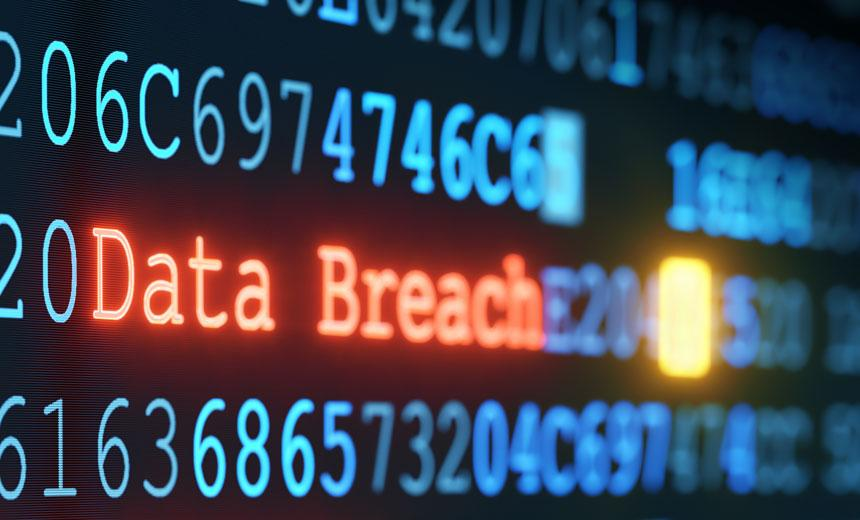
\includegraphics[width=\linewidth]{hack.jpg}
\end{figure}

\subsection{AOL (American Online)}
AOL was among the leading web portals and online service providers in the world Back in the early-to-mid-noughties. Then, almost at the peak of its powers, it was rocked by one of the most famous data breaches of the last fifteen years. AOL software engineer Jason Smathers used a colleague’s code to access the company’s screen name list in 2003 and stole the details of 92 million customer accounts including data like mails, ZIP codes, and credit card types. Smathers sold an updated version of the list to the 21-year-old Las Vegas-based online marketer Sean Dunaway for \$100,000 in 2004. In turn, Dunaway gave the spammers \$52,000. The email accounts hacked received over seven billion spam messages. \autocite{Breaches18}

\subsection{Yahoo}
Yahoo is one of the earliest pioneers of internet history. But its fortunes were on the wane when it got hit by what is by far the biggest of the biggest data breaches of all time in 2013-2014. An unidentified cybercriminal group successfully hacked all of Yahoo’s 3 billion accounts in August 2013. Hence, they gained access to a vast wealth of information, including names, email accounts, passwords, birth dates, phone numbers, and security questions and answers. Later, in August 2015, dark web sellers were offering lists containing 1 billion user account details for as much as \$300,000. An investigation then discovered that these lists included the names of 150,000 US government and military employees, as well as additional accounts related to the European Union, Canadian, British, and Australian governments.


\subsection{Target} 
Target is the eighth largest retailer in the US. On November 27, 2013, the attackers entered Target’s corporate network by taking the long route. They targeted a third-party vendor, refrigeration contractor Fazio Mechanical, with a spear-phishing attack. Then they gained control of Target’s services. They used malware to steal data from the company’s point of sale systems. According to Target’s official estimate, the personal and financial information of about 110 million credit/debit-card carrying customers had been compromised by one of the biggest data breaches in recent years. After this accident, Target tried to improve security by installing an application whitelisting POS systems, implementing POS management tools, and improving firewall rules and policies, among others.


\subsection{Blank Media Games}
Austin-based video game developer Blank Media Games is known for online browser game Town of Salem. Originally released in 2014, the game is based on the historic Salem witch trials, which resulted in the execution by hanging of nineteen people. An anonymous hacker stole the personal details of 7.6 million players, which includes usernames, passwords, email and IP addresses, game and forum activity, and purchased game premium features.

\subsection{Quora}
Quora is a popular question answer website. Quora observed some user data was accessed by third party on November 2018. That was data of over 100 million users including name ,email addresses, encrypted passwords, data from linked networks, public content and actions and finally  non-public content and actions, such as answer requests, upvotes, downvotes, and direct messages.

\subsection{Facebook}
Facebook engineers discovered a data breach on Tuesday, September 25, 2018, and patched it two days later.  Hackers managed to steal a type of digital security key which is known as access tokens. Data of over 50 million users including name, email addresses, encrypted passwords etc were accessed by the attackers. According to Facebook, the attack exploited three bugs that were present in the site’s “View as” feature from July 2017.  Facebook pushed 40 million users who had used the “View as” tool since July 2017 to log out, along with 50 million attacked accounts. As a consequence of this event, Facebook shares fell by about 3\%.

\subsection{Uber}
In October 2016, the hugely successful San Francisco-based ride-sharing startup, Uber, was attacked by hackers. This event affected about 7 million drivers and 50 million riders worldwide as well as 600,000 US driver’s license numbers. Hackers managed to get access of login information for an Uber Amazon Web Services account using a private GitHub site maintained by Uber engineers. They took 16 large files containing user information. Uber did not inform the regulation authority first, rather, it tried to manage the hackers by paying them \$100,000 to delete those data. 

\subsection{Linkedin}
LinkedIn is an American business and employment-oriented service that operates via websites and mobile apps, founded on December 28, 2002, and launched on May 5, 2003. In 2015, a Russian hacker group “Peace” stole almost 117 million Linkedin email and password combinations. They proceeded to offer the data on the dark web. 5 bitcoins or \$2,300 was the asking price. Linkedin asked all the affected users to change their passwords. They began encrypting and “salting” (adding random data to the passwords before they’re encrypted to make them less crackable) following an earlier hacking incident in 2012. \autocite{Breaches18}

\section{How Companies Use User Data}
Online services has a big collection of data to make benefits for everyone in many areas of life. But 
companies and other institutions can easily use their data wealth against people.\\
\\
\begin{figure}[h!]
 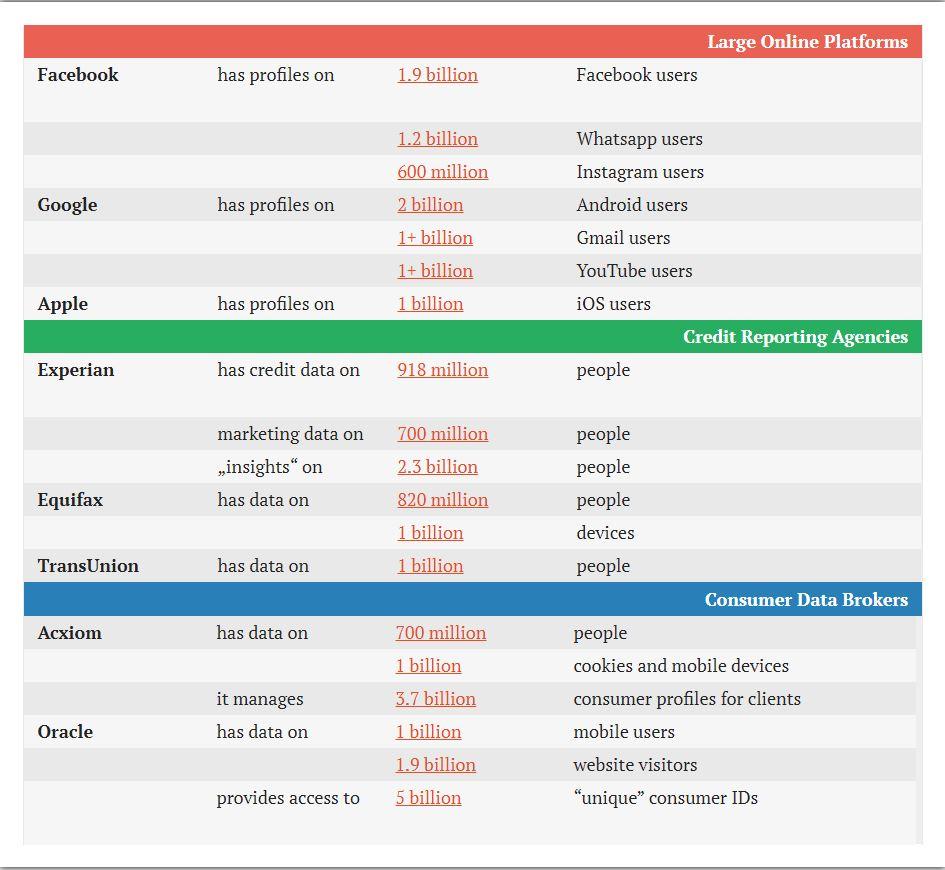
\includegraphics[height=11cm,width=\linewidth]{Capture.jpg}
\end{figure}
 The possible adverse effects of corporate data collection and utilization on individuals, groups of people, and society are diverse, but rarely considered in the commercial sphere. \\

Companies make decision about what service is to provide which user. They do it based on customer’s activities, choices, likes, comments, shared contents etc. This is to improve services and provide the best experience to user. \\
\\
Automated decision making systems exist with a view to treat people differently on the basis of information about them. As a result, individuals get excluded from certain opportunities, become subject to further investigation, or are filtered out in advance. Decisions whether to provide loans, insurance, health care, housing, education are taken based on those information. Fees and payment rates are also decided from here. \autocite{valentino2012websites} Data driven decisions may be taken as fully automated manners. As in banks, application for debit, credit, loans, can be denied and people can be automatically rated low. If there is inaccurate, persons can be mistreated. So there can occur technically inaccurate, intentionally biased decisions. \\
\\
Now a days, online social platforms, advertising agencies and online businesses in all industries can now monitor, recognize, and analyze individuals in many situations. They have information about what people are interested in, what they did today, what they are likely to do tomorrow, and how much they might be worth as a customer. Consumer data brokers and other firms have long been collecting information on newspaper and magazine subscribers, book and movie club members, catalog and mail order buyers, travel agency bookers, seminar and conference participants, and consumers filling out warranty cards, product registrations. The collection of purchase data from loyalty programs has also long been an established practice in this regard. \\
\\
Social Networking platform Facebook uses at least 52,000 personal attributes to categorize its 1.9 billion users by their political views, ethnicity, and income. To do such, the platform analyzes their posts, likes, shares, friends, photos, movements, and many other kinds of behaviors. In 2017, a leaked internal Facebook document revealed how the platform provides an advertiser the opportunity to target 6.4 million young Australians in “moments when young people need a confidence boost” such as when they felt “worthless”, “insecure”, “stressed”, “defeated”, “anxious”, or like a “failure”\autocite{tiku2017get}. Facebook claimed that it was not to use for advertising target users.  Similarly, the ride-hailing platform Uber has not only been accused of abusing its data power to manipulate both its drivers and riders, but also to identify, block, and undermine regulators, suppliers, and rivals. \autocite{calo2017taking} Facebook collects data about its users from other companies. This platform began its partnership in 2013 with the four data brokers Acxiom, Epsilon, Datalogix and BlueKai, the latter two of which were subsequently acquired by the IT giant Oracle.\\
\\
Companies also calculate scores to predict a person’s possible future behavior, with regard to, for example, someone’s economic stability or plans to have a baby or to change jobs. Even companies analise from the user profile and other user related to him, what is the health codition, probable diseases and health costs. \\
\\
Some companies make map about an individual’s movement, where he is going, staying and all about this. An interactive map can be made with hidden third-party tracking services on Android apps. \\
\\
Smartphones are the biggest contributors to today’s ubiquitous data collection. The information recorded by mobile phones provides detailed insights into a user’s personality and everyday life. Since consumers generally need to have a Google, Apple, or Microsoft account to use them, much of the information is already linked to a major platform’s identifier. From some years, companies began to make ways to combine and link digital profiles across platforms, customer databases, and the world of online advertising. The user information are used to influence user’s choice to have or purchase any service.\\
\\
Political manipulation is also done by using online platform’s data. The practice of targeting voters with personalized messages adapted to their personality and political views on certain issues has already raised massive debates about the potential for political manipulation. According to a Trump campaign official, the US presidential campaign in 2016 had “three major voter suppression operations under way that targeted white liberals, young women, and African-Americans with Facebook posts that portrayed Hillary Clinton as racist\autocite{halpern2017he}, thereby making her appear less appealing to these groups. \\
\\
\section{Conclusion}
Basically, this paper focused on big companies or institution who have a vast amount of user profile of people all around the world. In this paper, study on different types of encryption techniques is done. Some data breaches incidents happened so far have been studied also. Later, how companies use user data is explored. Companies use data to give better services as well as to bias and classify users.\\


\printbibliography

\end{document}